\documentclass[border=3pt]{standalone}
\usepackage{tikz}
\usetikzlibrary{arrows}

\definecolor{maincolor2}{RGB}{21,182,184}
\definecolor{qqqqff}{RGB}{1,82,142}
\definecolor{xdxdff}{RGB}{21,182,184}
\definecolor{eqeqeq}{rgb}{0.88,0.88,0.88}
\definecolor{ffxfqq}{rgb}{1,0.5,0}
\definecolor{cqcqcq}{rgb}{0.75,0.75,0.75}

\begin{document}
	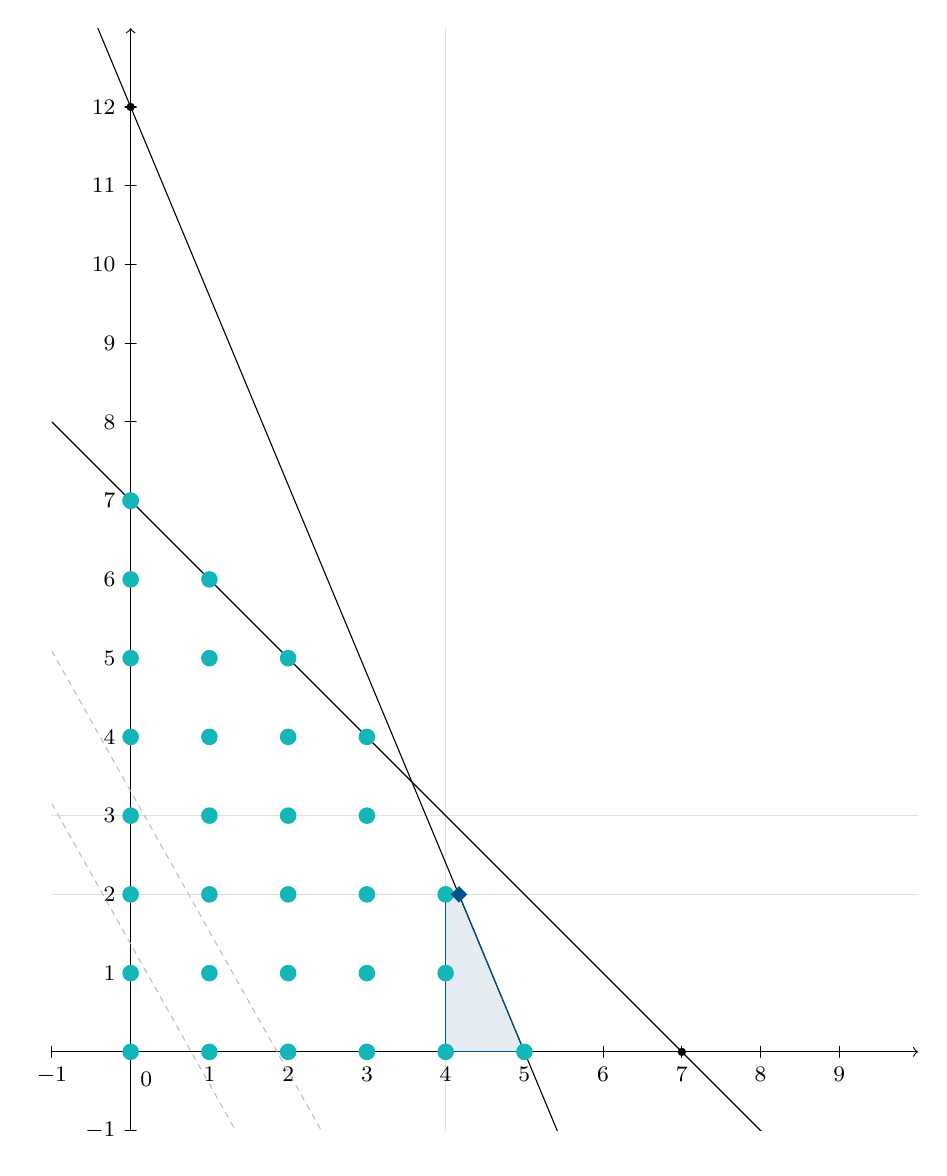
\begin{tikzpicture}[line cap=round,line join=round,x=1.0cm,y=1.0cm]
		\draw [line width=0.4pt,color=eqeqeq] (4,-1) -- (4,13);
		\draw [line width=0.4pt,color=eqeqeq,domain=-1:10] plot(\x,{(-2-0*\x)/-1});
		\draw [line width=0.4pt,color=eqeqeq,domain=-1:10] plot(\x,{(-3-0*\x)/-1});
		\draw[->,color=black] (-1,0) -- (10,0);
		\foreach \x in {-1,1,2,3,4,5,6,7,8,9}
		\draw[shift={(\x,0)},color=black] (0pt,2pt) -- (0pt,-2pt) node[below] {\footnotesize $\x$};
		\draw[->,color=black] (0,-1) -- (0,13);
		\foreach \y in {-1,1,2,3,4,5,6,7,8,9,10,11,12}
		\draw[shift={(0,\y)},color=black] (2pt,0pt) -- (-2pt,0pt) node[left] {\footnotesize $\y$};
		\draw[color=black] (0pt,-10pt) node[right] {\footnotesize $0$};
		\clip(-1,-1) rectangle (10,13);
		\fill[color=qqqqff,fill=qqqqff,fill opacity=0.1] (5,0) -- (4,0) -- (4,2) -- (4.17,2) -- cycle;
		\draw [domain=-1:10] plot(\x,{(--60-12*\x)/5});
		\draw [domain=-1:10] plot(\x,{(--49-7*\x)/7});
		\draw [dash pattern=on 2pt off 2pt,color=cqcqcq,domain=-1:10] plot(\x,{(--1.37-1.78*\x)/1});
		\draw [dash pattern=on 2pt off 2pt,color=cqcqcq,domain=-1:10] plot(\x,{(--3.31-1.78*\x)/1});
		\draw [color=qqqqff] (5,0)-- (4,0);
		\draw [color=qqqqff] (4,0)-- (4,2);
		\draw [color=qqqqff] (4,2)-- (4.17,2);
		\draw [color=qqqqff] (4.17,2)-- (5,0);
		\begin{scriptsize}
			\fill [color=black] (0,12) circle (1.5pt);
			\fill [color=maincolor2] (5,0) circle (3.0pt);
			\fill [color=maincolor2] (0,7) circle (3.0pt);
			\fill [color=black] (7,0) circle (1.5pt);
			\fill [color=maincolor2] (0,0) circle (3.0pt);
			\fill [color=maincolor2] (0,5) circle (3.0pt);
			\fill [color=maincolor2] (0,4) circle (3.0pt);
			\fill [color=maincolor2] (0,3) circle (3.0pt);
			\fill [color=maincolor2] (1,1) circle (3.0pt);
			\fill [color=maincolor2] (1,2) circle (3.0pt);
			\fill [color=maincolor2] (1,3) circle (3.0pt);
			\fill [color=maincolor2] (1,4) circle (3.0pt);
			\fill [color=maincolor2] (1,5) circle (3.0pt);
			\fill [color=maincolor2] (2,4) circle (3.0pt);
			\fill [color=maincolor2] (2,3) circle (3.0pt);
			\fill [color=maincolor2] (2,2) circle (3.0pt);
			\fill [color=maincolor2] (2,1) circle (3.0pt);
			\fill [color=maincolor2] (3,1) circle (3.0pt);
			\fill [color=maincolor2] (4,1) circle (3.0pt);
			\fill [color=maincolor2] (4,2) circle (3.0pt);
			\fill [color=maincolor2] (3,2) circle (3.0pt);
			\fill [color=maincolor2] (3,3) circle (3.0pt);
			\fill [color=maincolor2] (3,4) circle (3.0pt);
			\fill [color=ffxfqq] (-3.92,10.28) circle (4.5pt);
			\draw[color=ffxfqq] (-3.73,10.68) node {$J_1$};
			\fill [color=maincolor2] (0,2) circle (3.0pt);
			\fill [color=maincolor2] (0,1) circle (3.0pt);
			\fill [color=maincolor2] (1,0) circle (3.0pt);
			\fill [color=maincolor2] (2,0) circle (3.0pt);
			\fill [color=maincolor2] (3,0) circle (3.0pt);
			\fill [color=maincolor2] (4,0) circle (3.0pt);
			\fill [color=maincolor2] (0,6) circle (3.0pt);
			\fill [color=maincolor2] (1,6) circle (3.0pt);
			\fill [color=maincolor2] (2,5) circle (3.0pt);
			\fill [color=maincolor2] (0,7) circle (3.0pt);
			\fill [color=qqqqff] (4.17,2) ++(-3.0pt,0 pt) -- ++(3.0pt,3.0pt)--++(3.0pt,-3.0pt)--++(-3.0pt,-3.0pt)--++(-3.0pt,3.0pt);
		\end{scriptsize}
	\end{tikzpicture}
\end{document}